\documentclass[12pt]{article} % use larger type; default would be 10pt

\usepackage{pgfplots}
\usetikzlibrary{calc}
\usetikzlibrary{arrows}
\usetikzlibrary{patterns}
\usetikzlibrary{calc,intersections,through,backgrounds}
\usetikzlibrary{decorations.pathreplacing}
        \usepackage{xcolor} 
        \newcommand\degree[0]{^{\circ}}
        \newcommand\abs[1]{\left|#1\right|}
\usepackage{amsmath}
        \newcommand{\alert}[1]{\boldsymbol{\color{magenta}{#1}}}
        \newcommand{\blert}[1]{\boldsymbol{\color{blue}{#1}}}

\title{Play with TikZ}
\author{Just Us}
%\date{} % Activate to display a given date or no date (if empty),
         % otherwise the current date is printed 

\begin{document}
\maketitle

\section{Chap 7 Section 1}





hp-7-1-7 square

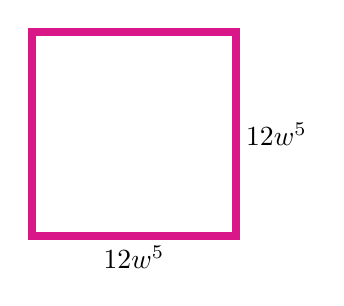
\begin{tikzpicture} 
\draw[magenta!90!black, line width=1mm] (0,0) rectangle ++(2.6,2.6);
\node[right] at (2.6,1.3) {$12w^5$};
\node[below] at (1.3,0) {$12w^5$};
\end{tikzpicture}
\newline



hp-7-2-8 rectangle

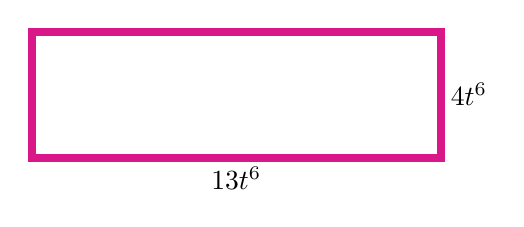
\begin{tikzpicture} [scale=.8]
\draw[magenta!90!black, line width=1mm] (0,0) rectangle ++(6.5,2.);
\node[right] at (6.5,1.) {$4t^6$};
\node[below] at (3.25,0) {$13t^6$};
\end{tikzpicture}
\newline


hp-7-2-9 subdivided rectangle

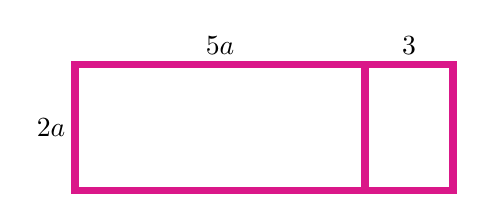
\begin{tikzpicture} [scale=.8]
\draw[magenta!90!black, line width=1mm] (0,0) rectangle ++(6,2.);
\draw[magenta!90!black, line width=1mm] (4.6,0) --++(0,2);
\node[above] at (2.3,2) {$5a$};
\node[above] at (5.3,2) {$3$};
\node[left] at (0,1) {$2a$};
\end{tikzpicture}
\newline


hp-7-2-10 subdivided rectangle

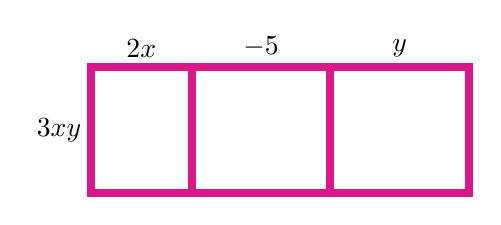
\begin{tikzpicture} [scale=.8]
\draw[magenta!90!black, line width=1mm] (0,0) rectangle ++(6,2.);
\draw[magenta!90!black, line width=1mm] (1.6,0) --++(0,2);
\draw[magenta!90!black, line width=1mm] (3.8,0) --++(0,2);
\node[above] at (0.8,2) {$2x$};
\node[above] at (2.7,2) {$-5$};
\node[above] at (4.9,2) {$y$};
\node[left] at (0,1) {$3xy$};
\end{tikzpicture}
\newline


\section{Section 7.4}

hp-7-4-3

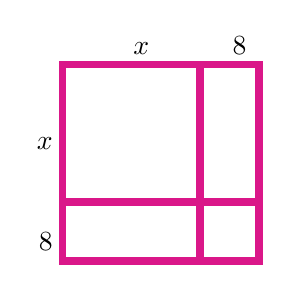
\begin{tikzpicture} 
\draw[magenta!90!black, line width=1mm] (0,0) rectangle ++(2.5,2.5);
\draw[magenta!90!black, line width=1mm] (0,.75) --++(2.5,0);
\draw[magenta!90!black, line width=1mm] (1.75,0) --++(0,2.5);
\node[above] at (1,2.5) {$x$};
\node[above] at (2.25,2.5) {$8$};
\node[left] at (0,1.5) {$x$};
\node[left] at (0,0.25) {$8$};
\end{tikzpicture}
\newline

hp-7-4-4

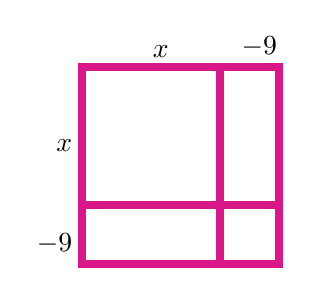
\begin{tikzpicture} 
\draw[magenta!90!black, line width=1mm] (0,0) rectangle ++(2.5,2.5);
\draw[magenta!90!black, line width=1mm] (0,.75) --++(2.5,0);
\draw[magenta!90!black, line width=1mm] (1.75,0) --++(0,2.5);
\node[above] at (1,2.5) {$x$};
\node[above] at (2.25,2.5) {$-9$};
\node[left] at (0,1.5) {$x$};
\node[left] at (0,0.25) {$-9$};
\end{tikzpicture}
\newline


hp-7-4-42 colored rectangles

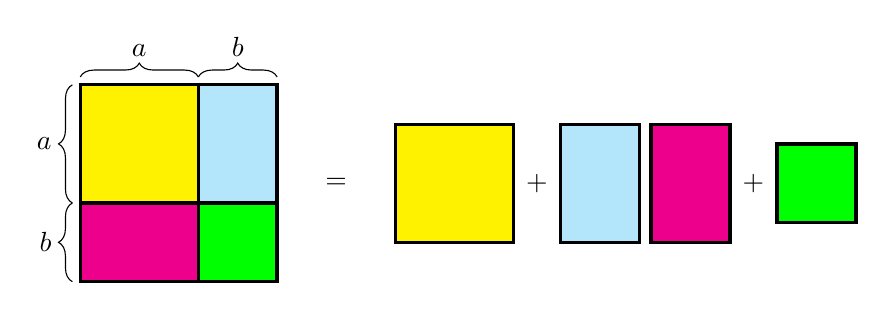
\begin{tikzpicture} 
\draw[black, fill=yellow, very thick] (0,1) rectangle (1.5,2.5);
\draw[black, fill=magenta, very thick] (0,0) rectangle ++(1.5,1);
\draw[black, fill=cyan!30!white, very thick] (1.5,1) rectangle (2.5,2.5);
\draw[black, fill=green, very thick] (1.5,0) rectangle ++(1,1);

\draw [black,decorate,decoration={brace,amplitude=5pt}] (0,1)++(-.1,0) -- ++(0,1.5) node [black, left,midway,xshift=-4pt] {$a$};
\draw [black,decorate,decoration={brace,amplitude=5pt}] (0,0)++(-.1,0) -- ++(0,1) node [black, left,midway,xshift=-4pt] {$b$};
\draw [black,decorate,decoration={brace,amplitude=5pt}] (0,2.5)++(0, .1) -- ++(1.5,0) node [black, above,midway,yshift=4pt] {$a$};
\draw [black,decorate,decoration={brace,amplitude=5pt}] (1.5,2.5)++(0, .1) -- ++(1,0) node [black, above,midway,yshift=4pt] {$b$};
\coordinate(O) at (3.25,1.25);
\node at (O) {$=$};
\coordinate(A) at (4,.5);
\draw[black,very thick, fill=yellow] (A) rectangle ++(1.5,1.5);
\node at ($(O)+(2.55,0)$) {$+$};
\draw[black,very thick, fill=cyan!30!white] (A)++(2.1,0) rectangle ++(1,1.5);
\draw[black,very thick, fill=magenta] (A)++(3.25,0) rectangle ++(1,1.5);
\node at ($(O)+(5.3,0)$) {$+$};
\draw[black,very thick, fill=green] (A)++(4.85,0.25) rectangle ++(1,1);
\end{tikzpicture}
\newline





\section{Section 7.4}





cr7-45 rectangle

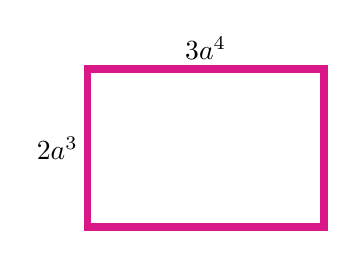
\begin{tikzpicture} 
\draw[magenta!90!black, line width=1mm] (0,0) rectangle ++(3,2);
\node[above] at (1.5,2) {$3a^4$};
\node[left] at (0,1) {$2a^3$};
\end{tikzpicture}
\newline


cr7-46 rectangle

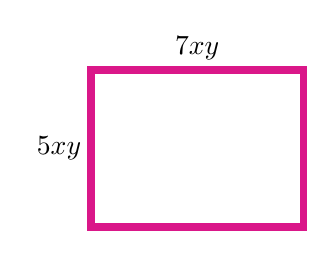
\begin{tikzpicture} 
\draw[magenta!90!black, line width=1mm] (0,0) rectangle ++(2.7,2);
\node[above] at (1.35,2) {$7xy$};
\node[left] at (0,1) {$5xy$};
\end{tikzpicture}
\newline


cr7-47 rectangle

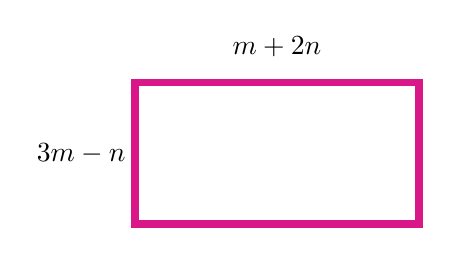
\begin{tikzpicture} 
\draw[magenta!90!black, line width=1mm] (0,0) rectangle ++(3.6,1.8);
\node[above] at (1.8,2) {$m+2n$};
\node[left] at (0,0.9) {$3m-n$};
\end{tikzpicture}
\newline


cr7-48 rectangle

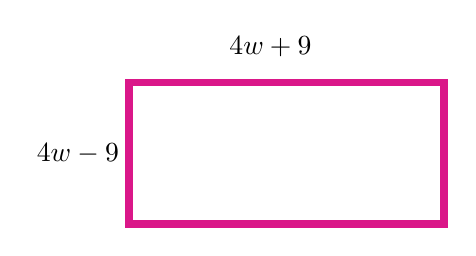
\begin{tikzpicture} 
\draw[magenta!90!black, line width=1mm] (0,0) rectangle ++(4,1.8);
\node[above] at (1.8,2) {$4w+9$};
\node[left] at (0,0.9) {$4w-9$};
\end{tikzpicture}
\newline



\section{Other stuff}

10 by 10 grid: hp-2-3-12

8 by 8 grid: hp-4-5-17

5-by-5 grid hp-6-4-9



\end{document}
